% Created 2021-02-05 Fri 17:40
% Intended LaTeX compiler: pdflatex
\documentclass[presentation]{beamer}
\usepackage[utf8]{inputenc}
\usepackage[T1]{fontenc}
\usepackage{graphicx}
\usepackage{grffile}
\usepackage{longtable}
\usepackage{wrapfig}
\usepackage{rotating}
\usepackage[normalem]{ulem}
\usepackage{amsmath}
\usepackage{textcomp}
\usepackage{amssymb}
\usepackage{capt-of}
\usepackage{hyperref}
\usetheme{UoB}
\author{Mark Blyth}
\date{\textit{[2021-02-05 Fri]}}
\title{Autonymous CBC}
\hypersetup{
 pdfauthor={Mark Blyth},
 pdftitle={Autonymous CBC},
 pdfkeywords={},
 pdfsubject={},
 pdfcreator={Emacs 27.1 (Org mode 9.3)}, 
 pdflang={English}}
\begin{document}

\maketitle

\section{Background}
\label{sec:orgee8d360}
\begin{frame}[label={sec:org2644f96}]{Week's activities}
\begin{itemize}
\item Implemented van der Pol (vdP) CBC with Fourier
\begin{itemize}
\item Doesn't work
\end{itemize}
\end{itemize}
\vfill
\begin{itemize}
\item Implemented adaptive-knots splines
\begin{itemize}
\item Requried to make BSpline CBC work with vdP
\end{itemize}
\end{itemize}
\vfill
\begin{itemize}
\item Implemented vdP CBC with BSplines
\begin{itemize}
\item Doesn't work
\end{itemize}
\end{itemize}
\vfill
\begin{itemize}
\item Read about practical bursters
\end{itemize}
\vfill
\begin{itemize}
\item Wrote some notes on discretisors
\end{itemize}
\end{frame}


\begin{frame}[label={sec:orge41fcce}]{Reading}
Read about why single cells don't burst but populations do
\begin{itemize}
\item Bursting requires quite specific parameter values
\item Real cells have enough variation in these parameters that it's rare to find one that can burst
\item Coupled cells can take on the dynamics of their averaged parameter values
\begin{itemize}
\item Individual cells rarely lie within the bursting parameter range
\item Collections of cells average out their parameter values and allow bursting
\end{itemize}
\end{itemize}
\vfill
Issue: bursts in networks are a bit messy
\begin{itemize}
\item Individual cells in the network no longer show nice neat bursts
\item Can't define any nice neat control target
\item Limits the scope to which CBC can be applied
\end{itemize}
\end{frame}

\begin{frame}[label={sec:orgb11a5cc}]{Noisy bursts}
\begin{center}
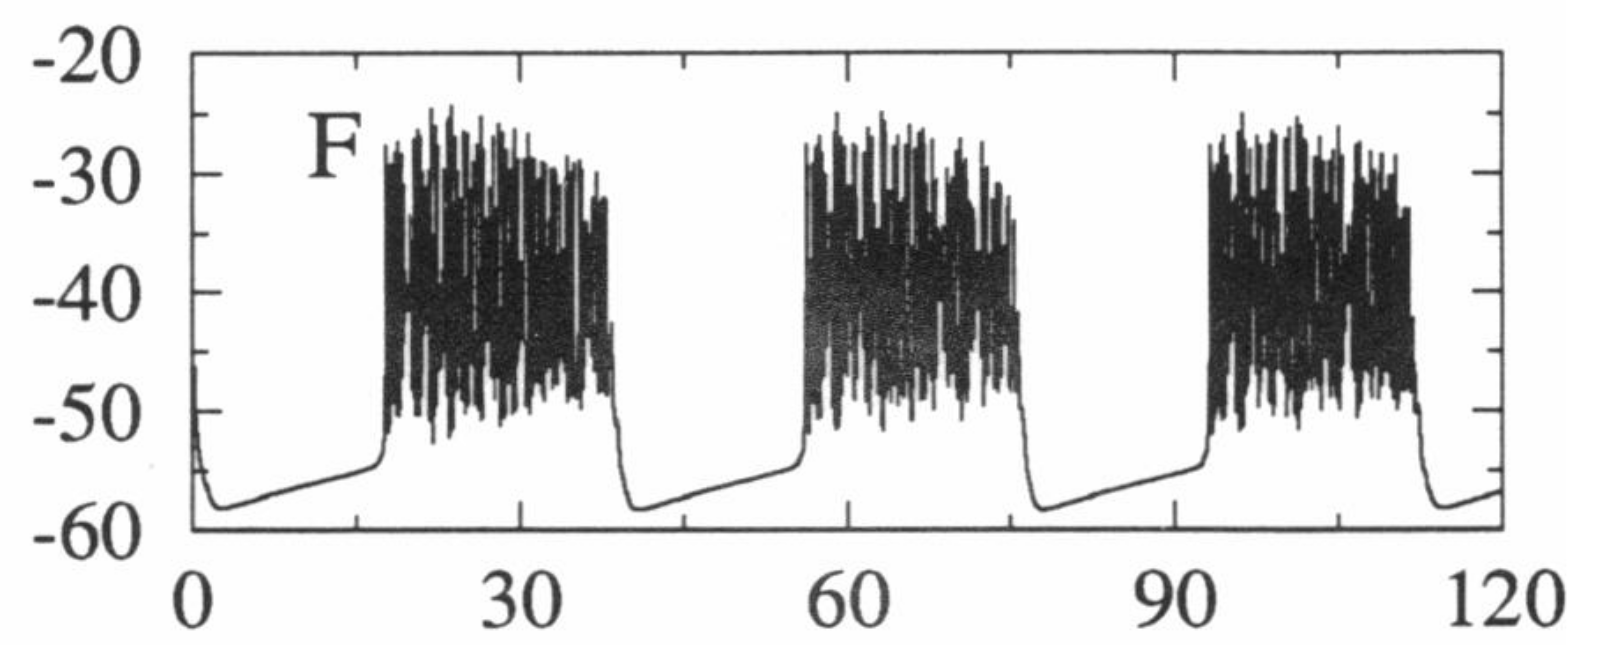
\includegraphics[width=.9\linewidth]{./burst.png}
\end{center}
\vfill
\begin{itemize}
\item These results are from simulations
\item Question for Krasi is how biologically realistic this is
\begin{itemize}
\item Can we ever get `nice' bursts in real cells?
\end{itemize}
\end{itemize}
\end{frame}


\section{Extended CBC}
\label{sec:org9899f34}
\begin{frame}[label={sec:org507bf4f}]{Autonymous CBC}
\begin{itemize}
\item Continuation vector contains parameter, period, discretisation
\begin{itemize}
\item Initialisation parameters chosen by user
\item Initialisation period determined by zero-crossings
\item Initialisation discretisation found by discretising uncontrolled system output at initial parameters
\end{itemize}
\end{itemize}
\vfill
\begin{itemize}
\item Continuation equations enforce\ldots{}
\begin{itemize}
\item Input discretisation = output discretisation
\item Pseudo-arclength condition
\item Integral phase condition, with previous accepted solution as a reference \(v(t)\)
\end{itemize}
\end{itemize}
\vfill
\[\Psi[x^*] = \int_0^1 \left\langle x^*\left(\frac{t}{T_{x^*}}\right),  \dot{v}\left(\frac{t}{T_v}\right) \right\rangle \mathrm{d}t\]
\end{frame}

\begin{frame}[label={sec:orgd605a04}]{Fourier vdP}
Not much benefit to nonadaptive-knots vdP BSpline CBC
\begin{itemize}
\item vdP signal is very nonlinear; nonadaptive would need lots of coefficients
\item If we're using lots, may as well use the simpler Fourier method
\end{itemize}
\vfill
Tested out vdP-Fourier
\begin{itemize}
\item Didn't work, Jacobian somehow ended up singular
\item SciPy solvers didn't work either
\end{itemize}
\vfill
Didn't put much effort into testing why this happens
\begin{itemize}
\item Splines would be easier to test
\begin{itemize}
\item Nicer numbers (consistently \(\mathcal{O}(1)\))
\item Fewer of them (lower-dimensional discretisation)
\end{itemize}
\item Decided to skip the numerics checking and jump straight to splines
\end{itemize}
\end{frame}

\begin{frame}[label={sec:org91031e6}]{Part 1: initialising adaptive knots}
BSplines need adaptive knots to be useful on vdP; this works as follows
\vfill
Choose good knots at initialisation
\begin{itemize}
\item Let \(\xi\) be a knot vector, \(x_0\) be the initialiser signal, \(\hat{x}(\xi)\) its least-squares spline approximation
\item Find \(\mathrm{argmin }\xi \quad \|x_0 - \hat{x}(\xi)\|_2^2\), over signal samples
\begin{itemize}
\item Initialise knots as uniformly distributed random variables
\item Numerically optimize
\item Repeat lots of times to avoid local minima
\item Choose the best result
\end{itemize}
\end{itemize}
\end{frame}

\begin{frame}[label={sec:orgdf1ac76}]{Part 2: Adapting the adaptive knots}
Knots are updated after each prediction/correction step
\vfill
\begin{itemize}
\item Initial knots will already be a good guess of optimal knots
\begin{itemize}
\item They were optimal for the previous signal
\item We assume optimal knot set changes smoothly with signal
\end{itemize}
\item Run a single optimization step
\begin{itemize}
\item Fit knots to the newly accepted output signal
\end{itemize}
\item Update current knots to newly optimized result
\end{itemize}
\end{frame}

\begin{frame}[label={sec:org8b28410}]{Part 3: Using adaptive knots}
Must re-discretise at each prediction/corrector step
\vfill
\begin{itemize}
\item Discretisation must be consistent between all vectors in any given prediction/corretion step
\item Take accepted solutions from previous two results and project on to the current knot set
\item Use the rediscretised solutions for secant prediction
\end{itemize}
\vfill
Goodness-of-fit of each knot optimization result gives us a good check that the discretisation is still valid
\begin{itemize}
\item If goodness-of-fit becomes bad, we might need more knots in the discretisation
\item I hold discretisation size fixed, but it could easily be varied
\end{itemize}
\end{frame}

\begin{frame}[label={sec:orgfe217db}]{Adaptive-BSpline autonymous CBC}
It doesn't work very well

\begin{center}
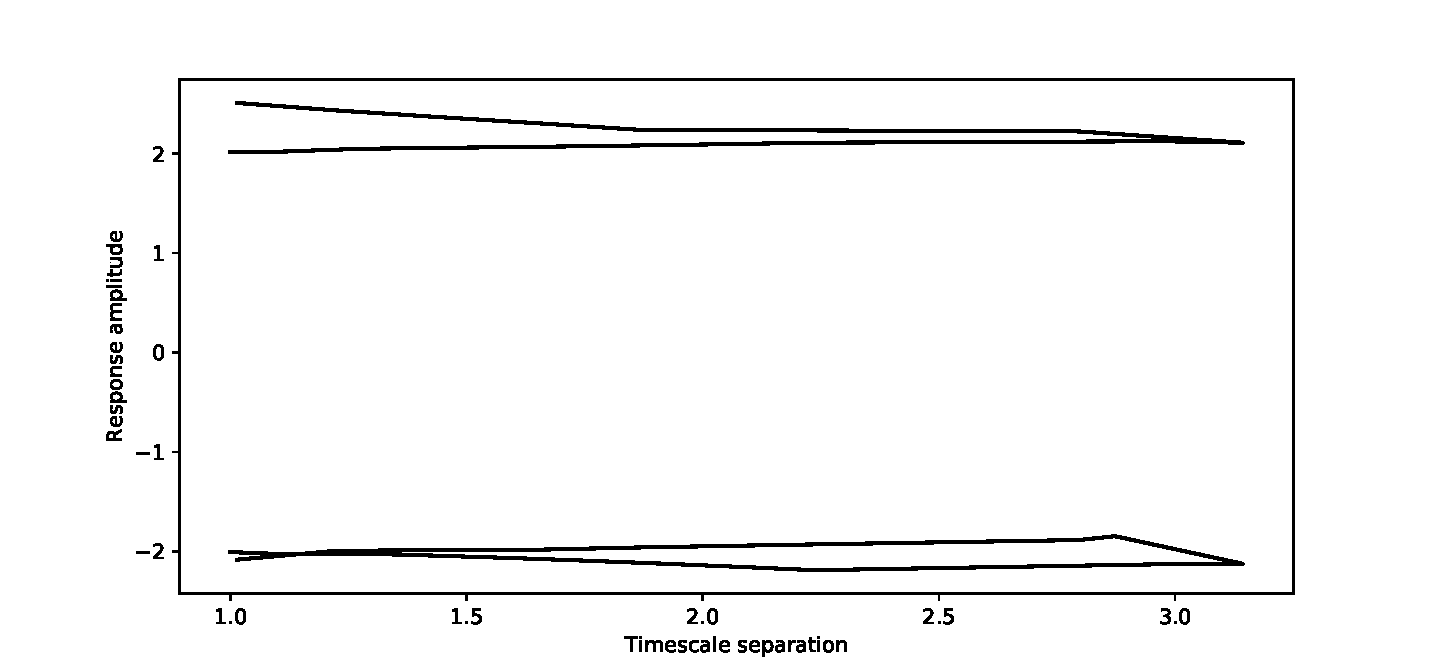
\includegraphics[width=.9\linewidth]{./fail.pdf}
\end{center}
\end{frame}

\begin{frame}[label={sec:org130ae56}]{Possible issues and improvements}
Code is only just finished
\begin{itemize}
\item Haven't had time to test stepsizes, Jacobian methods, solvers, etc.
\item Might be as simple as a different stepsize
\end{itemize}
\end{frame}

\begin{frame}[label={sec:orgd5d5052}]{Phase constraints}
Maybe the continuation equations aren't very good?
\begin{itemize}
\item No particular reason why Galerkin projections should be robust at estimating period
\begin{itemize}
\item Counter-argument: it's worked fine for other people!
\end{itemize}
\item Phase constraint makes the coefficients similar to their previous values; doesn't encode anything particularly interesting or meaningful
\begin{itemize}
\item Must be specified to get a unique solution, however doesn't encode anything interesting; doesn't help us find a solution in a numerically robust way
\end{itemize}
\end{itemize}
\vfill
\begin{itemize}
\item Collocation is a good way to find oscillation periods
\begin{itemize}
\item Keeps extending a solution boundary around the limit cycle, until it finds the period that makes the two boundaries meet
\item Phase constraint encodes where to put one of the boundaries
\end{itemize}
\end{itemize}
\vfill
Collocation might be a generally more robust way of doing things
\end{frame}

\section{Next steps}
\label{sec:org5260373}
\begin{frame}[label={sec:org5f4b524}]{Next steps}
\begin{itemize}
\item Play some more with the code and see if anything interesting can be made to happen
\item If it can't, try collocation instead
\item Also, keep reading and writing
\end{itemize}
\end{frame}
\end{document}
